The source code in {\tt amrex/Src/Amr} contains a number of classes, most notably
{\tt Amr}, {\tt AmrLevel}, and {\tt LevelBld}.
These classes provide a more well developed set of tools for writing AMR codes
than the classes created for the {\tt Advection\_AmrCore} tutorial.
\begin{itemize}
\item The {\tt Amr} class is derived from {\tt AmrCore}, and manages data across the 
entire AMR hierarchy of grids.
\item The {\tt AmrLevel} class is a pure virtual class for managing data at a
single level of refinement.
\item The {\tt LevelBld} class is a pure virtual class for defining variable types
and attributes.
\end{itemize}

Many of our mature, publicly application codes contain derived classes that inherit directly
from {\tt AmrLevel}.  These include our compressible astrophysics code,
{\tt CASTRO},
(available in the {\tt AMReX-Astro/Castro} github repository) 
 and our computational cosmology code, {\tt NYX}
(available in the {\tt AMReX-Astro/Nyx} github repository)   .
Our incompressible Navier-Stokes code, {\tt IAMR}
(available in the {\tt AMReX-codes/IAMR} github repository)
has a pure virtual class called {\tt NavierStokesBase} that inherits from {\tt AmrLevel},
and an additional derived class {\tt NavierStokes}.
Our low Mach number combustion code {\tt PeleLM} (not yet public) also inherits
from {\tt NavierStokesBase}.

The tutorial code in {\tt amrex/Tutorials/Amr/Advection\_AmrLevel} gives a simple
example of a class derived from {\tt AmrLevel} that can be used to solve
the advection equation on a subcycling-in-time AMR hierarchy.  Note that example
is essentially the same as the {\tt amrex/Tutorials/Amr/Advection\_AmrCore} tutorial
and documentation in Chatper \ref{Chap:AmrCore}, except now we use the provided
libraries in {\tt Src/Amr}.

The tutorial code also contains a {\tt LevelBldAdv} class (derived from {\tt LevelBld} in the
{\tt Source/Amr} directory).  This class is used to define variable types (how many, nodality,
interlevel intepolation stencils, etc.).

The most important data managed by the {\tt AmrLevel} is an array of {\tt StateData},
which holds the scalar fields, etc., in the boxes that together make up the level.

\section{{\tt StateData}}
{\tt StateData} is a class that essentially holds a pair of {\tt MultiFab}s: one at the old time and one
at the new time. {\tt AMReX} knows how to interpolate in time between these states to get data at
any intermediate point in time. The main data that we care about in our applications codes 
(such as the fluid state) will be stored as {\tt StateData}. Essentially, data is made {\tt StateData}
if we need it to be stored in checkpoints / plotfiles, and/or we want it to be automatically
interpolated when we refine.
An {\tt AmrLevel} stores an array of {\tt StateData} (in a C ++ array called state). We index this array
using integer keys (defined via an enum in, e.g., {\tt AmrLevelAdv.H}):
\begin{lstlisting}[language=cpp]
enum StateType { Phi_Type = 0,
                 NUM_STATE_TYPE };
\end{lstlisting}
In our tutorial code, we use the function {\tt AmrLevelAdv::variableSetup} to tell our simulation about
the {\tt StateData} (e.g., how many variables, ghost cells, nodality, etc.)
Note that if you have more than one {\tt StateType}, each of the different {\tt StateData} 
carried in the state array can have different numbers
of components, ghost cells, boundary conditions, etc. This is the main reason we separate all this
data into separate {\tt StateData} objects collected together in an indexable array.

\section{{\tt Advection\_AmrLevel} Example}

Figure \ref{fig:AmrAdvection_AmrLevel_flowchart} shows a source
code tree for the {\tt AmrAdvection\_AmrLevel} example.
%%%%%%%%%%%%%%%%%%%%%%%%%%%%%
\begin{figure}[htb]
\begin{center}
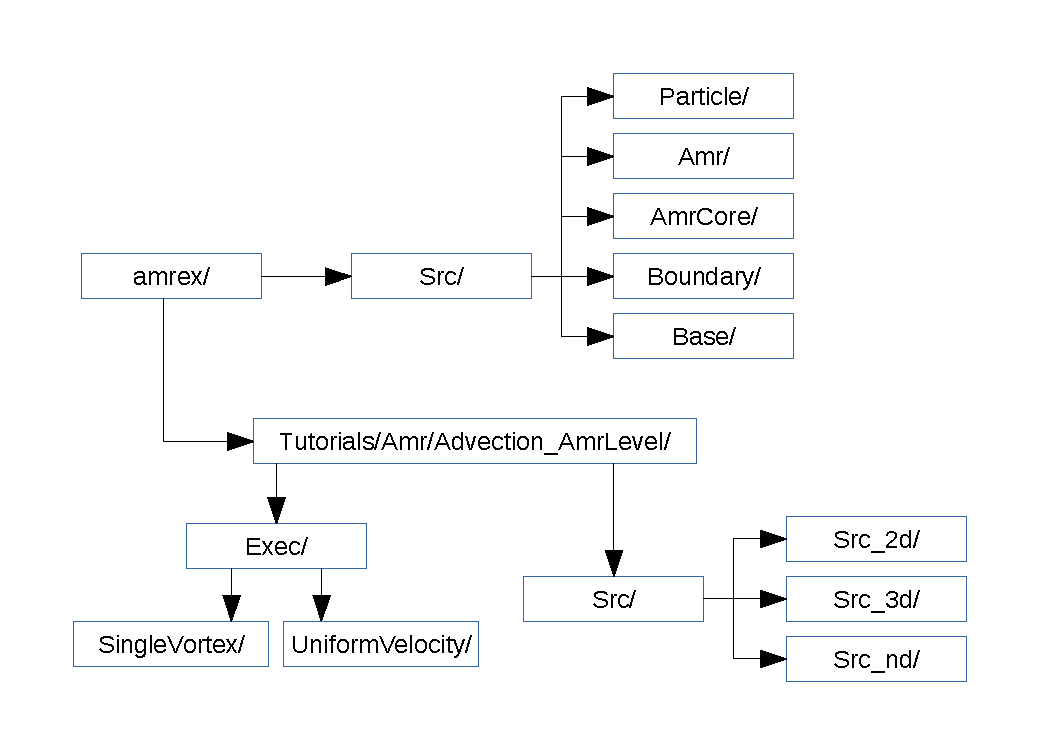
\includegraphics[width=4in]{./AmrLevel/figs/flowchart.pdf}
\caption{\label{fig:AmrAdvection_AmrLevel_flowchart} Source code tree for the 
         {\tt AmrAdvection\_AmrLevel} example.}
\end{center}
\end{figure}
%%%%%%%%%%%%%%%%%%%%%%%%%%%%%
\begin{itemize}
\item {\tt amrex/Src/}
\begin{itemize}
\item {\tt Base/} Base {\tt amrex} library.
\item {\tt Boundary/} An assortment of classes for handling boundary data.
\item {\tt AmrCore/} AMR data management classes, described in more detail above.
\item {\tt Amr/}
\item {\tt Particle/}
\end{itemize}
\item {\tt Advection\_AmrLevel/Src} Source code specific to this example.  Most notably
is the {\tt AmrLevelAdv} class, which is derived from {\tt AmrLevel}.  The subdirectories {\tt Src\_2d}
and {\tt Src\_3d} contain dimension specific routines.  {\tt Src\_nd} contains dimension-independent routines.
\item {\tt Exec} Contains a makefile so a user can write other examples besides {\tt SingleVortex} and {\tt UniformVelocity}.
\item {\tt SingleVortex} and {\tt UniformVelocity}
Build the code here by editing the {\tt GNUmakefile} and running {\tt make}.  There
is also problem-specific source code here used for initialization or specifying the velocity field used in this
simulation.
\end{itemize}

\begin{lstlisting}[language=cpp]
/* Advection_AmrLevel Pseudocode */
main()
  Amr amr;
  amr.init()
  loop { 
    amr.coarseTimeStep()
      /* compute dt */
      timeStep()
        amr_level[level]->advance()
        /* call timeStep r times for next-finer level */
        amr_level[level]->post_timestep() // AMR synchronization
      postCoarseTimeStep()
      /* write plotfile and checkpoint */
  }
  /* write final plotfile and checkpoint */
\end{lstlisting}
